\documentclass[12pt]{scrartcl}
\usepackage[sexy]{james}
\usepackage[noend]{algpseudocode}
\setlength {\marginparwidth}{2cm}
\usepackage{answers}
\usepackage{array}
\usepackage{tikz}
\newenvironment{allintypewriter}{\ttfamily}{\par}
\usepackage{listings}
\usepackage{xcolor}
\usetikzlibrary{arrows.meta}
\usepackage{color}
\usepackage{mathtools}
\newcommand{\U}{\mathcal{U}}
\newcommand{\E}{\mathbb{E}}
\usetikzlibrary{arrows}
\Newassociation{hint}{hintitem}{all-hints}
\renewcommand{\solutionextension}{out}
\renewenvironment{hintitem}[1]{\item[\bfseries #1.]}{}
\renewcommand{\O}{\mathcal{O}}
\declaretheorem[style=thmbluebox,name={Chinese Remainder Theorem}]{CRT}
\renewcommand{\theCRT}{\Alph{CRT}}
\setlength\parindent{0pt}
\usepackage{sansmath}
\usepackage{pgfplots}

\usetikzlibrary{automata}
\usetikzlibrary{positioning}  %                 ...positioning nodes
\usetikzlibrary{arrows}       %                 ...customizing arrows
\newcommand{\eqdef}{=\vcentcolon}
\newcommand{\tr}{{\rm tr\ }}
\newcommand{\im}{{\rm Im\ }}
\newcommand{\spann}{{\rm span\ }}
\newcommand{\Col}{{\rm Col\ }}
\newcommand{\Row}{{\rm Row\ }}
\newcommand{\dint}{\displaystyle\int}
\newcommand{\dt}{\ {\rm d }t}
\newcommand{\PP}{\mathbb{P}}
\newcommand{\horizontal}{\par\noindent\rule{\textwidth}{0.4pt}}
\usepackage[top=3cm,left=3cm,right=3cm,bottom=3cm]{geometry}
\newcommand{\mref}[3][red]{\hypersetup{linkcolor=#1}\cref{#2}{#3}\hypersetup{linkcolor=blue}}%<<<changed

\tikzset{node distance=4.5cm, % Minimum distance between two nodes. Change if necessary.
         every state/.style={ % Sets the properties for each state
           semithick,
           fill=cyan!40},
         initial text={},     % No label on start arrow
         double distance=4pt, % Adjust appearance of accept states
         every edge/.style={  % Sets the properties for each transition
         draw,
           ->,>=stealth',     % Makes edges directed with bold arrowheads
           auto,
           semithick}}


% Start of document.
\newcommand{\sep}{\hspace*{.5em}}

\pgfplotsset{compat=1.18}
\begin{document}
\title{AMSC460: Computational Methods}
\author{James Zhang\thanks{Email: \mailto{jzhang72@terpmail.umd.edu}}}
\date{\today}

\definecolor{dkgreen}{rgb}{0,0.6,0}
\definecolor{gray}{rgb}{0.5,0.5,0.5}
\definecolor{mauve}{rgb}{0.58,0,0.82}

\lstset{frame=tb,
  language=Java,
  aboveskip=3mm,
  belowskip=3mm,
  showstringspaces=false,
  columns=flexible,
  basicstyle={\small\ttfamily},
  numbers=left,
  numberstyle=\tiny\color{gray},
  keywordstyle=\color{blue},
  commentstyle=\color{dkgreen},
  stringstyle=\color{mauve},
  breaklines=true,
  breakatwhitespace=true,
  tabsize=3
}


\maketitle
These are my notes for UMD's CMSC460: Computational Methods. These notes are taken live in class 
(``live-\TeX``-ed). This course is taught by Professor Haizhao Yang. The textbook for the course is 
\textit{A First Course in Numerical Methods} by OU Ascher and Chen Greif.
\tableofcontents

\newpage

\section{Scientific Computing}

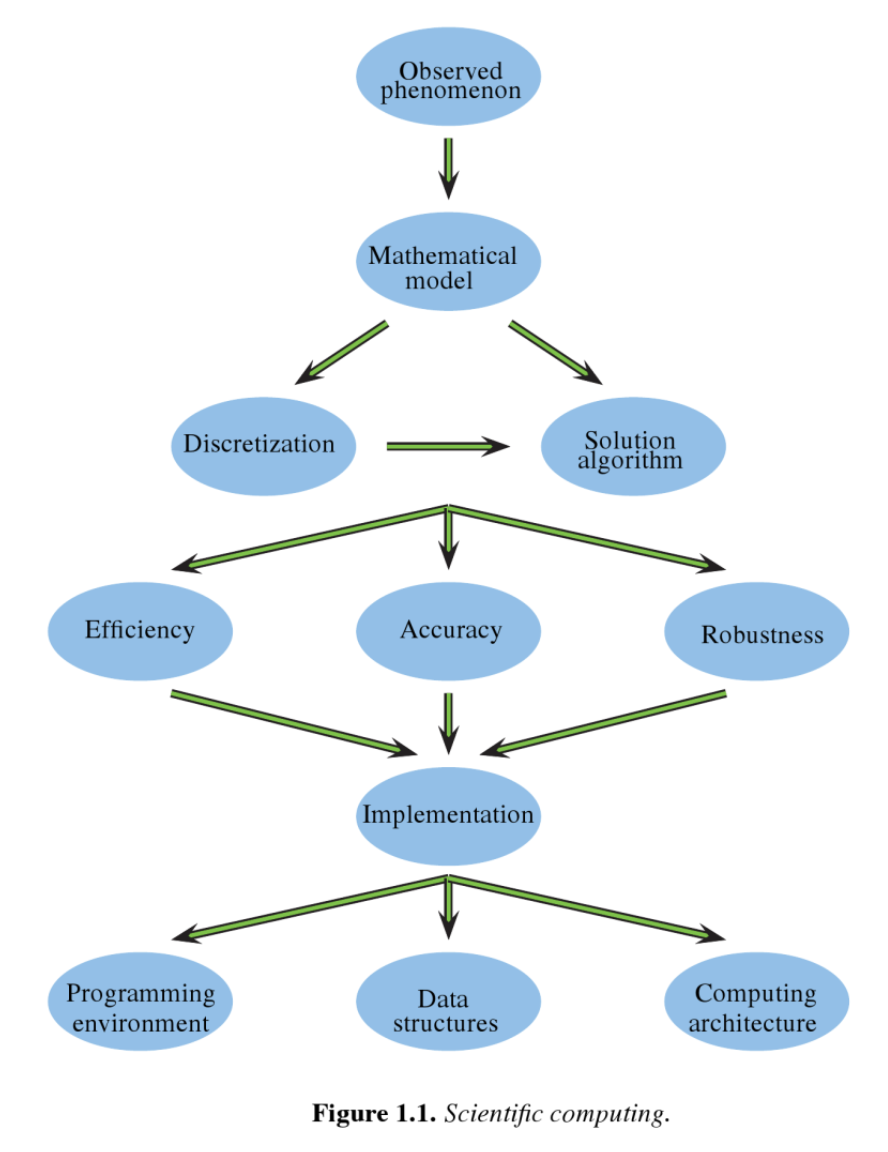
\includegraphics[width=10cm]{scientific_compute.png}

\begin{definition}[Relative and Absolute Errors]
  Let the target value be $u \in \RR$ and let the numerical solution be $v \in \RR$, then the 
  \vocab{absolute error} is $|u-v|$ and the \vocab{relative error} is $\frac{|u-v|}{|u|}$.
\end{definition}

\begin{note}
If $|u|$ is large, then relative error is used and if $|u|$ is very small, then relative error 
is not a good measurement.
\end{note}

\begin{example}[The Stirling Approximation]
  The formula $u = S_n = \sqrt{2\pi n} \cdot(\frac{n}{e})^n$ is used to approximate $n!$.
  \begin{lstlisting}[language=Matlab]
    e = exp(1);
    n = 1 : 10;
    # Note that the following are vectors of len 10.
    S_n = sqrt(2*pi*n).*((n/e).^n);
    # Compute absolute and relative err.
    fact_n = factorial(n);
    abs_err = abs(fact_n - S_n);
    rel_err = abs_err./abs(fact_n);
    format short g
    [n; fact_g; abs_err; real_err;]'
  \end{lstlisting}
\end{example}

\subsection{Numerical Algorithms and Errors}

\begin{definition}[Error Types]

  \hfill

  \begin{enumerate}
    \item Error in the problem to be solved. These may be errors in the mathematical model or errors in the input data.
    \item Approximation errors, which can consist of discretization errors (errors in interpolation, differentiation, integration) or 
    convergence errors, which can also arrive in iterative methods
    \item Roundoff errors
  \end{enumerate}
\end{definition}

\begin{definition}[Taylor Series]
  Assume that $f(x)$ has $k+1$ derivatives in an interval containing the point $x_0$ and 
  $x_0 + k$. Then 
  \[f(x_0 + k) = f(x_0) + hf'(x_0)+ \frac{h^2}{2} + \cdots + \frac{h^k}{k!}f^{(k)}(x_0) + \frac{h^{k+1}}{(k+1)!}f^{(k+1)}(\xi)\]
  where $\xi$ is some point between $x_0$ and $x_0 + h$, and the term $\frac{h^{k+1}}{(k+1)!}f^{(k+1)}(\xi)$ is the remainder term.
\end{definition}

\begin{note}
  To find $f'(x_0)$ observe that 
  \[f'(x_0) = \frac{f(x_0 + k) - f(x_0)}{h}\] 
  and then if we take the limit of this 
  \[f'(x_0) = \lim_{h\to 0} \frac{f(x_0 + k) - f(x_0)}{h}\]
  we recover the $h$-definition of a derivative, and the discretization error is 
  $\frac{h}{2}f''(\xi)$ because our model is 
  \[hf'(x_0) = f(x_0 + k) - f(x_0) - \frac{h^2}{2}f''(x_0) + \cdots\]
  \[\implies f'(x_0) = \frac{f(x_0 + k) - f(x_0)}{h} - \left(\frac{h}{2}f''(x_0) + \cdots\right)\]
  \[\implies \left| f'(x_0) - \frac{f(x_0 + k) - f(x_0)}{h} \right| = \left| \frac{h}{2}f''(x_0) + \cdots \right|\]
\end{note}

\begin{definition}[Big-$\mathcal{O}$ and $\Theta$ Notation]
  We define these for error characterization in terms of some parameters.
  \[\begin{cases}
    h \text{ represents a small parameter }\\
    n \text{ represents a large parameter }
  \end{cases}\]
\end{definition}

\begin{note}
  An error $e$ depending on $h$ we denote $e = \mathcal{O}(h^q)$ and if there are two positive constants 
  $q$ and $C$ such that 
  \[|e| \leq Ch^q\]
  Similarly, we write $e = \Theta(h^q)$ if $\ \exists \ C_1, C_2$ and $q > 0$
  such that 
  \[C_1h^q \leq |e| \leq C_2h^q\]
  $n$ represents the problem size and then we use big $\O$ and $\Theta$ to denote the time or memory complexity of an algorithm.
\end{note}

\begin{example}
  If we say $T = \Theta(n\log n)$ then we find $C_1, C_2, x_0$ such that 
  \[C_1n\log n \leq T \leq C_2n \log n \ \forall \ x \geq x_0\]
\end{example}

\begin{note}
    
  Note that errors go down and then back up as $h$ changes. A small number divided by another small number is a dangerous,
  think about exploding and vanishing gradients when training neural networks.

  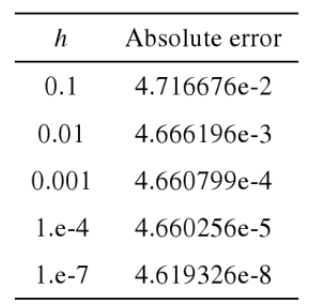
\includegraphics[width=6cm]{good.png}
  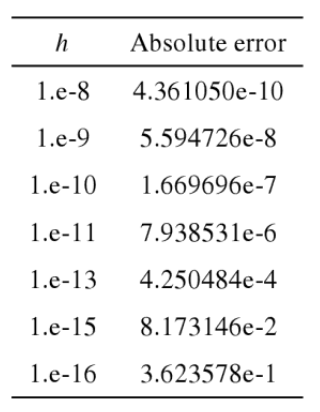
\includegraphics[width=5cm]{bad.png}
  
\end{note}

\begin{note}
  In practice, error is the sum of \vocab{discretization error} + \vocab{rounding error}
\end{note}

\subsection{Algorithm Properties}

Some good assessments of the quality of an algorithm are accuracy, efficiency, and robustness

\begin{definition}[Accumulated Error]
  Suppose you're evaluating polynomial with large degree. Your error $e_1$ from $p_1$ gets compounded 
  by $e_2$ from $p_2$ and so on and so forth, so the total error follows
  \[\text{Total error } \leq |e_1| + \cdots + |e_n|\]
\end{definition}

\subsection{Binary Representation, Rounding Errors, Truncation Errors}

\begin{remark}
  Math claim: Any real number $x \in \RR$ is accurately representable by an infinite sequence of digits, eg. $x \approx \pm 1$
  \[x = \pm c(1.\{d_1\}\ldots\{d_{t+1}\}\cdots) \times 2^e\]
  where $d_1, d_2, \cdots$ are integer numbers $0$ or $1$, and $e$ is the integer exponent.

  For each $e$, you can find a sequence to represent this real number $x$. 
\end{remark}

\begin{example}
  Let $x = -(1.10110\cdots) \times 2^1$ which means $x = -1 + 1 \times \frac{1}{2} + 0 \times \frac{1}{2^2} + 1 \times \frac{1}{2^3} + \cdots$
  where the $\frac{1}{2^t}$ term, we denote as $\frac{1}{s^t}$
\end{example}

\begin{definition}[Truncating]
  Chopping ignores digits $d_t, d_{t+1}, \cdots$ yielding $\overset{\sim}{x} = \pm (1.\{d_1\}\cdots\{d_{t-1}\}) \times 2^e \approx x$
  and so the error is $\O(\frac{1}{2^{te}}) = \O(\frac{1}{s^t})$
\end{definition}

\section{Roundoff Errors}

\begin{definition}[Binary Floating Point Representations]
  Infinite sequence representing $x \in \RR$
  \[x = \pm C(1.d_1 d_2 d_3 \cdots) \times 2^e\]
  where $e$ is an integer chosen to make $d_0$ not $0$. The $1.d_1d_2\cdots$ is known as the 
  \vocab{mantissa}.

  For example: $x = 2^{12} \implies e = 12, x = (1.00\cdots) \times e^{12}$
\end{definition}

\begin{note}
  Note that $d_0 = 1$ always in binary representations because we have restrictions that $d_0 \neq 1$, which we will see later.
\end{note}

\begin{note}[Geometric Understanding]
  A real number $\implies$ infinite sequence. For binary, if $x \in (1, 1.5)$ then choose 
  $d_1 = 0$. If $x \in (1.25, 1.5)$, choose $d_1 = 1$. For all $x \in \RR,$ you can always find 
  $2^e$ such that $\frac{x}{2^e} \in [1, 2]$. 

  For example: $x = 1 + 2^{12} \implies 2^e = 2^{12} \implies \frac{1 + 2^{12}}{2^{12}} \in [1, 2]$ and 
  $x = 2^{-5} + 2^{-4} \implies 2^e = 2^{-4} \implies \frac{2^{-5} + 2^{-4}}{2^{-4}} \in [1, 2]$
\end{note}

\begin{note}
  To get a real number from the infinite sequence, use the equation 
  \[(1.d_1d_2\cdots) \times 2^e = (1 + \frac{d_1}{2} + \frac{d_2}{4} + \cdots) \times 2^e\]
\end{note}

\begin{note}
  A general floating point representation is denoted as 
  \[fl(x) = \text{sign}(x) \times (1.\hat{d}_1 \hat{d}_2 \cdots) \times 2^e\]
  where $\hat{d}_i$ is determined by $d_i$. Because of truncation, we have errors and this is called 
  rounding errors or machine accuracy.
\end{note}

\subsection{Floating Point Systems}

\begin{definition}
  A floating point system can be characterized by a 4-tuple $(\beta, t, L, U)$ where 
  \begin{itemize}
    \item $\beta$ is the base of the number system 
    \item $t = $ precision, or the number of digits
    \item $L$ is the lower bound on the exponent $e$
    \item $U$ is the upper bound on the exponent $e$ 
  \end{itemize}
  This definition leads to a generalization of floating point representations 
  \[fl(x) = \sign{x} \left( \frac{\overset{\sim}{d}_0}{\beta_0} + \frac{\overset{\sim}{d}_1}{\beta_1} + \cdots\right) \times \beta^e\]
  where $0 \leq \overset{\sim}{d}_i < \beta - 1$ and $e$ is chosen such that $\overset{\sim}{d}_0 \neq 0$.
\end{definition}

\begin{definition}[Chopping]
  Ignore $d_t, \cdots$ yielding $\overset{\sim}{d}_i = d_i$ and 
  
  $fl(x) = \pm (d_0.d_1d_2\cdots d_{t-1}) \times \beta^e$
\end{definition}

\begin{definition}[Rounding]
  Consult $d_t$ to determine the approximation 
  \[fl(x) = \begin{cases}
    \pm (d_0.d_1d_2d_3\cdots d_{t-1}) \times \beta^1 \text{ if } d_t < \frac{\beta}{2}\\
    \pm (d_0.d_1d_2d_3\cdots d_{t-1} + \beta^{1-t}) \times \beta^e \text{ otherwise }
  \end{cases}\]
  Essentially, we consider what we want to keep and discard. Note that the next term would be $\frac{d_t}{\beta_t} \times \beta^e$
\end{definition}

\begin{example}
  Consider $x = \frac{8}{3} = 2.66\cdots \in \RR$
  \[x = (\frac{2}{10^0} + \frac{6}{10^1} + \cdots) \times 10^0\]
  $\beta = 10, e = 0$ so that $d_0 \neq 0$

  \begin{itemize}
    \item We can chop this so that $t = 4$ in which case 
    \[fl(x) = (\frac{2}{10^0} + \frac{6}{10^1} + \frac{2}{10^2} + \frac{6}{10^3}) \times 10^0 = 2.666\]
    \item Or we can round this so that $t = 4$ in which case since $d_t = 6 > \frac{\beta}{2} = 5$ we have 
    \[fl(x) = (\frac{2}{10^0} + \frac{6}{10^1} + \frac{2}{10^2} + \frac{6}{10^3} + 10^{1-4}) \times 10^0 = 2.667\]
  \end{itemize}
\end{example}

\begin{theorem}[Floating Point Representation Error]
  Absolute error 
  \[|x - fl(x)| \leq \begin{cases}
    \beta^{1-t} \ \cdot \ \beta^1 \text{ for chopping } \\
    \frac{1}{2}\beta^{1-t} \ \ cdot \ \beta^1 \text{ for rounding }
  \end{cases}\]
  and relative error 
  \[\frac{|x - fl(x)|}{|x|} \leq \begin{cases}
    \beta^{1-t} \text{ for chopping } \\
    \frac{1}{2}\beta^{1-t} \text{ for rounding }
  \end{cases}\]
\end{theorem}

\subsection{Errors in Computation}


\begin{note}

\hfill

\begin{enumerate}
  \item $x + y$ may have large absolute error if $x >> y$
  \item If $|y| << 1$, then $\frac{x}{y}$ may have large relative and 
  absolute error 
  \item $xy$ is dangerous if $y$ is large
  \item If $x \approx y$ then $x - y$ has large relative error 
  \[\text{relative error} = \frac{|v - (x-y)|}{|x-y|}\]
  due to the denominator being small
\end{enumerate}
\end{note}

\begin{definition}[Overflow and underflow]
  An \vocab{overflow} means a number is too large too fit into the floating point system $\implies e > U$. 
  an \vocab{underflow} means a number has $e < L$, where $L$ is a large negative number. 

  Example: $L = -14, e = -15, \beta = 10$, $\beta^e = 10^{-15}$ is what you want, but
  $\beta^L = 10^{-14}$ is the smallest case the computer can compute. So, the computer will round it at zero. 
\end{definition}

\section{Nonlinear Equations in One Variable}

\begin{definition}[Question 1 in this Section]
  Given a nonlinear function $f(x)$ and an interval $[a,b]$, find a root 
  denoted as $x^*$ if it exists on $[a,b] \implies$ find $f(x^*) = 0$. On Matlab, you can use the 
  \vocab{\textit{fzero}} function
\end{definition}

\begin{note}
  Discontinuous functions may not have a root. Similarly, $e^x > 0 \ \forall \ x$, even though this 
  function is continuous.
\end{note}

\begin{note}[Intermediate Value Theorem]
  If $f(u)$ and $f(v)$ change signs, then by the Intermediate Value Theorem, we have least one root on $[a,b]$ if 
  $f(x)$ is continuous. 
\end{note}

\begin{definition}[Question 2 in this Section]
  Do we have a unique root? 

  Example: Linear equations in most cases have one root, whereas nonlinear equations may have multiple roots.
  If we have multiple roots, how can we design an algorithm to find the desired root?
\end{definition}

\subsection{Iterative Methods to Find Roots}

\begin{definition}
  We have a sequential decision-making process to produce
  \[X_0 \to X_1 \to X_2 \to X_3 \to \cdots \to X_n \cdots\]
  until we have found a sufficiently good $X_n$. Some things we need to think about. 
  \begin{itemize}
    \item How do we initialize $X_0$?
    
    Changing signs to find $[a,b]$, if $a=b$ then any point in $[a,b]$ is good?
    You can also draw the function to get some good $x_0$

    \item How to move from $X_n$ to $X_{n+1}$

      
    \item When do we stop?

    \begin{enumerate}
      \item If $|f(X_n)| < \text{ftol}$
      \item If $|X_n - X_{n-1}| < \text{atol} \approx 0$
      \item If $X_n - X_{n-1}| < \text{rtol} \approx 0$
      \item If $n > $ max iterations then quit.
    \end{enumerate}

  \end{itemize}
\end{definition}

\begin{note}[Desired Properties of an Algorithm]

  \hfill

  \begin{enumerate}
    \item Efficiency (small number of iterations, cheap computation per iteration, cheap memory per iteration)
    \item Robustness
    \item Minimum requirement of $f(x)$
    \item Generalizable to other questions
  \end{enumerate}
  
\end{note}

\subsection{Bisection Method}

\begin{definition}[Bisection Method]
  Suppose $f(x)$ changes sign on an interval $[a,b]$. By the Intermediate Value Theorem, 
  we know there exists a root $x^* \in [a,b]$. Now evaluate $p = \frac{a+b}{2}$, or the midpoint.
  and check the sign of $f(a) \cdot f(p)$. If this product is negative, then the root is in $[a, p]$ and so set $b \leftarrow p$. Else, the 
  root is in $[p, b]$ and so set $a \leftarrow p$. Repeat. 
\end{definition}

\begin{note}
  If we repeat this computation, we will have $[a_0, b_0] \supset [a_1, b_1] \supset \cdots \supset [a_n, b_n] \supset \cdots$
  then 
  \[\lim_{n\to\infty} a_n = \lim_{n\to\infty} = x^*\]
  the root of $f(x)$.
\end{note}

\subsection{Fixed Point Iteration}

\begin{definition}[Fixed Point Iteration]
  A fixed point denoted as $x^*$ of a function $g(x)$ is the point that satisfies 
  \begin{align*}
    g(x^*) = x^*
  \end{align*}
  Problem reformulation: Identifying a root of $f(x)$ is reformulated into a problem of identifying a fixed point of $g(x)$
\end{definition}

\begin{example}
    Ex 1: $g(x) = x - f(x)$ then $g(x^*) = x^* \implies x^* = x^* - f(x^*) \implies f(x^*) = 0$

    Ex 2: $g(x) = \frac{x - f(x)}{f'(x)} \implies x^* = x^* - \frac{f(x^*)}{f'(x^*)} \implies \frac{f(x^*)}{f'(x^*)} = 0 \implies f(x^*) = 0$

    We want to look at our problem and choose $g$ such that it is easy to find $x^*$ such that $f(x^*) = 0$
\end{example}

\begin{note}[How do we find a fixed point?]
  Let's try to obtain a geoemtric understanding of the problem.

  \begin{center}
    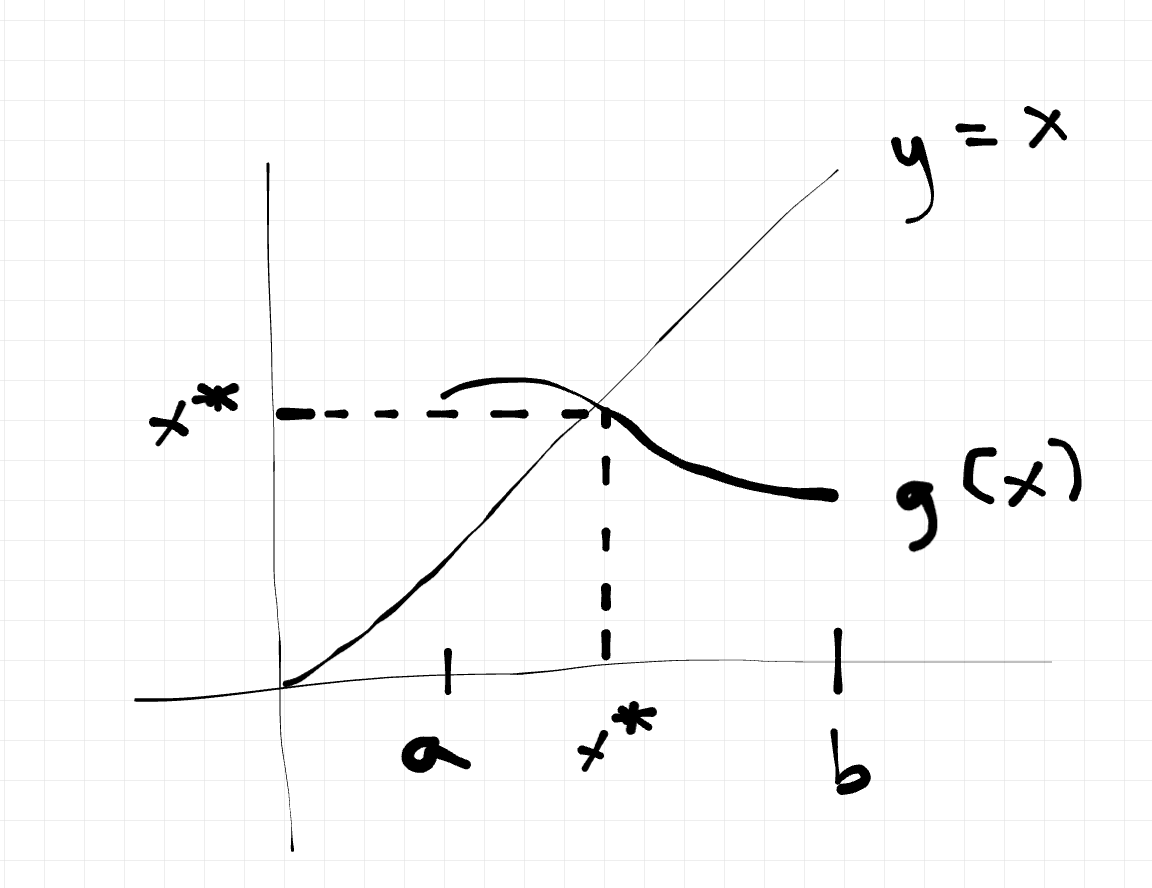
\includegraphics[width=7cm]{geo.png}
    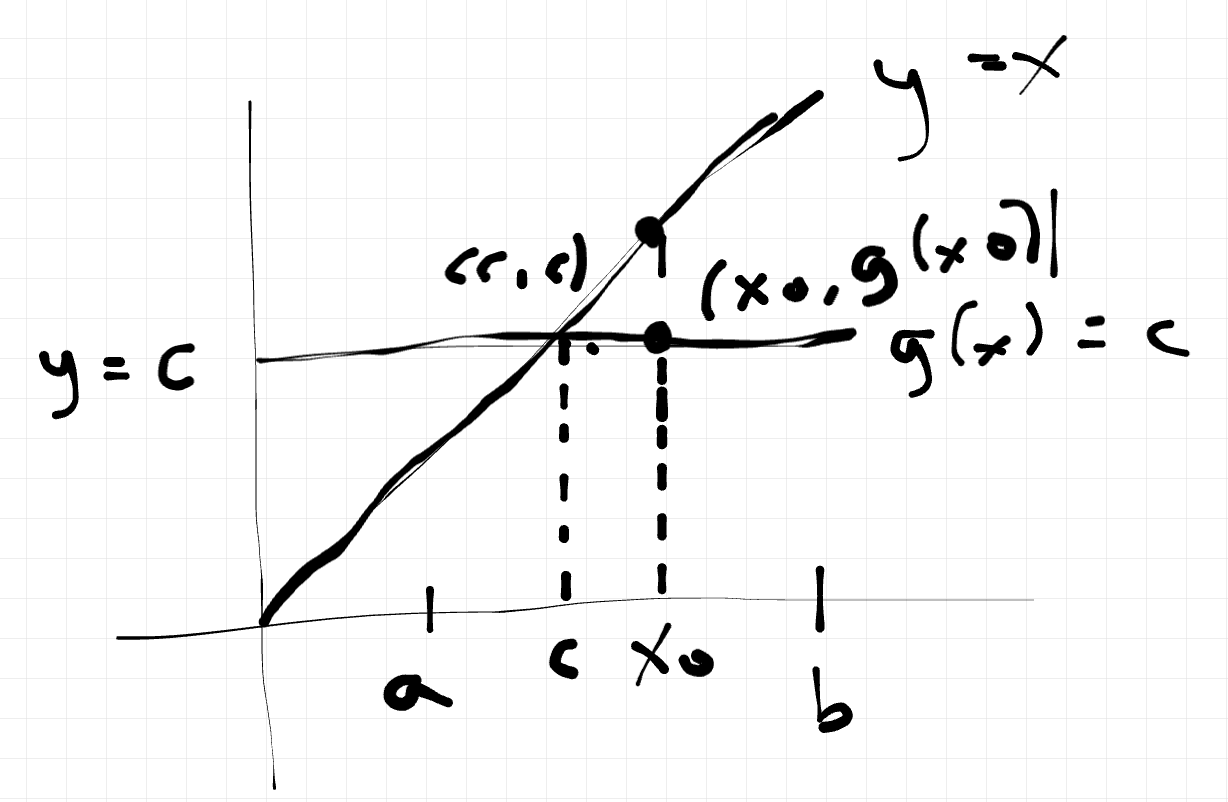
\includegraphics[width=7cm]{gconstant.png}
  \end{center}

  Start at an initial guess $x_0$, then evaluate $g(x_0)$ and set up an improved guess 
  \[x_1 = g(x_0) = c\]
  then surprisingly $x_1$ is the fixed point $x^*$.
  \[g(x_1) = g(c) = c = x_1 \implies g(x_1) = x_1\]
  and therefore $x_1$ is a fixed point. So, in the special case, $g(x)$ is a constant, 
  the iteration rule $x_{k+1} = g(x_k)$ gives a fixed point after one iteration. 
\end{note}

\begin{note}
  Conjecture: we use $x_{k+1} = g(x_k)$ as an updating rule to generate a sequence $\{x_k\}$ for a general 
  $g(x)$. We have $\underset{k\to\infty}{x_k} \to x^*$ under certain conditions.
\end{note}

\begin{definition}[Fixed Point Algorithm]
  Given $f(x)$, select a function $g(x)$ after an appropriate reformulation.

  \begin{enumerate}
    \item Start from an initial guess $x_0$
    \item For $k = 0, 1, 2, \cdots$ set $x_{k+1} = g(x_k)$ until $x_{k+1}$ satisfies a termination criteria.
  \end{enumerate}
\end{definition}

\begin{note}[Questions for Fixed Point Iteration]
  Some important things to note about fixed point iteration

  \begin{enumerate}
    \item Is there a fixed point $x^*$ on $[a,b]$?
    
    \begin{proof}
      The proof for this is very similar to the proof of the existence of a root, it follows 
      naturally from the Intermediate Value Theorem. 
    \end{proof}
    \item If yes, what about convergence?
    
    The fixed point is not necessarily unique ie. imagine a curve that oscillates repeatedly around $g(x)$. 
    So $g'(x)$ is a good property to use to study the fixed point iteration. If $g(x) = c \longleftrightarrow g'(x) = 0$, 
    $x_1 = g(x_0)$ gives a fixed point $x^* = x_1$ with only one step.

    If $g(x)$ changes a lot (ie. $|g'(x)|$) large, then fixed point iteration may be wrong. 
    So, we conejcture that if $|g'(x)|$ is small, we can prove that $x_k \to x^*$
    
    \item Does $x_k \to x^*$?

      Assume that $|g'(x) \leq \rho$ on $[a,b]$. Then we can prove uniqueness and convergence  

      \begin{proof}
        
        Uniqueness: suppose we have two fixed points $x_1^*, x_2^*$ on $[a,b]$. The following 
        first step is by definition of fixed points, then apply Taylor Series First Order Approximation
        \[|x_1^* - x_2^*| = |g(x_1^*) - g(x_2^*)| = |g'(\xi)(x_1^* - x_2^*)| \leq \rho|x_1^* - x_2^*|\]
        Note that we have shown that $|x_1^* - x_2^*| \leq \rho |x_1^* - x_2^*|$. If $\rho > 1$, then this doesn't show 
        us anything useful. If $\rho < 1$, then this is only satisfied if $|x_1^* - x_2^*| = 0 \implies x_1^* = x_2^*$.

        \hfill

        Convergence: 
        \[x_{k+1} - x^*| = |g(x_k) - g(x^*)| = |g'(\xi)(x_k - x^*) \leq \rho(x_k - x^*)|\]
        and so 
        \[|x_{k+1} - x^*| \leq \rho |x_k - x^*| \leq \rho^2 |x_{k-1} - x^*|| \leq \cdots \leq \rho^{k+1}|x_0 - x^*||\]
        \[\lim_{k\to\infty} |x_{k+1} - x^*| = 0\]
      \end{proof}
    
    \item If yes, how fast does $x_k \to x^*$?
    
      This is a contraction by the faster $\rho$, the smaller $\rho$ is, the faster the convergence 
      \[\text{rate} = -\log_{10}(\rho)\]

  \end{enumerate}
\end{note}

\subsection{Newton's Method}

\begin{note}
  
  \hfill

  \begin{center}
    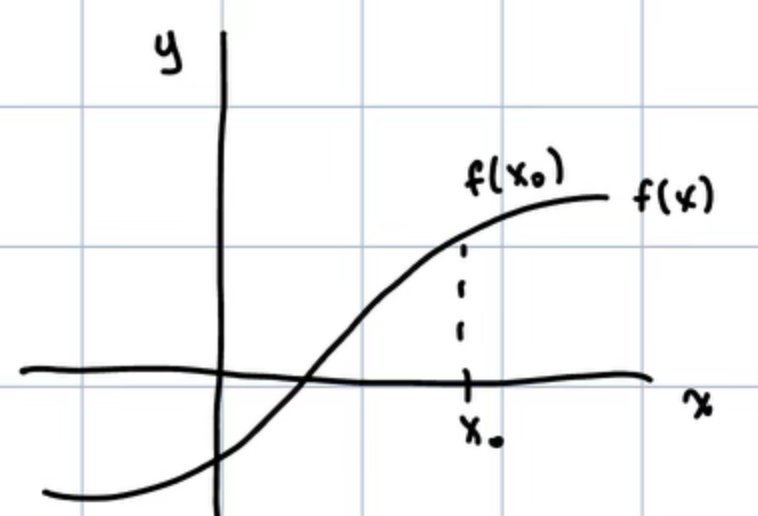
\includegraphics[width=10cm]{newtons.png}
  \end{center}
\end{note}

\begin{definition}[Analytic Understanding of Newton's Method]
  Consider the First Order Taylor Series expansion of $f(x)$ 
  \[f(x) = f(x_k) + f'(x_k)(x-x_k) + \frac{f''(\xi(x))}{2}(x-x_k)^2\]
  where $\xi$ is between $x$ and $x_k$. 
  $f'(x_k) = \frac{f(x_k)}{x_k - x_{k+1}}$ is a linear equation in $x_{k+1}$
  \[\Leftrightarrow (x_k - x_{k+1})f'(x_k) = f(x_k)\]
  \[\Leftrightarrow f(x_k) + (x_{k+1} - x_k)f'(x_k) = 0\]
  \[x_{k+1} = x_k - \frac{f(x_k)}{f'(x_k)}\]
  and this is the updating rule to get $x_{k+1}$ which is closer to $x^*$ than $x_k$. 
  This is the Newton's Method to generate a sequence of $\{x_k\}$. 
\end{definition}

\begin{definition}[Newton's Method as an Algorithm]
  \hfill

  \begin{enumerate}
    \item Start from an initial guess $x_0$.
    \item FOr $k = 0, 1, 2, \ldots,$ set 
    \[x_{k+1} = x_k - \frac{x_k}{f'(x_k)}\]
    until $x_{k+1}$ satisfies the termination criteria.
  \end{enumerate}
\end{definition}

\begin{note}[Local Convergence]
  If you don't start with a sufficiently good $x_0$, you may not have $\underset{k\to\infty}{x_k} = x^*$
\end{note}

\begin{note}[Global Convergence]
  To find $x_0$ good enough to ensure convergence, plot the graph and start in a neighborhood 
  near-ish a root. (what?)
\end{note}

\begin{note}[How Fast is Convergence?]
  \hfill

  \begin{enumerate}
    \item Recall that for fixed point iteration, convergence is dependent on $\rho$ 
  \[|x_{k+1} - x^*| \leq p|x_k - x^*|\]
  this is called \vocab{linear convergence} because the right hand side is a linear function of the error term $|x_k - x^*|$. 
    \item On the other hand, Newton's Method has \vocab{quadratic convergence}
    \[|x_{k+1} - x^*| \leq M|x_k - x^*|^2\]
    Typically, we do'n't go above this (ie. to cubic convergence) due to the increase of computing resources
    \item \vocab{Superlinear convergence}: if $\exists \ \{\rho_k\}, \rho_k \to 0$ such that 
    \[|x_{k+1} - x^*| \leq \rho_k|x_k - x^*| \leq \rho|x_k - x^*|\]
    Note that superlinear convergence implies linear convergence, and it may or may not be quadratic convergence,
    but quadratic convergence is always superlinear convergence.
  \end{enumerate}
\end{note}

\subsection{Secant Method - Variant of Newton's Method}

\begin{definition}
  Consider a First Order Taylor Series Expansion once more
  \[f(x) \approx f(x_0) + f'(x_0)(x-x_0) \implies f'(x_0) \approx \frac{f(x) - f(x_0)}{x-x_0}\]
  \[\implies f'(x_k) \approx \frac{f(x_k) - f(x_{k-1})}{x_k - x_{k-1}}\]
  \[\implies x_{k+1} = x_k - \frac{f(x_k)}{\frac{f(x_k) - f(x_{k-1})}{x_k - x_{k-1}}} = x_k - \frac{f(x_k)(x_k - x_{k-1})}{f(x_k) - f(x_{k-1})}\]
\end{definition}

\begin{note}[Secant Method as an Algorithm]
  \hfill

  \begin{enumerate}
    \item Start from an educated guess $x_0$
    \item For $k = 0, 1, 2, \cdots$ set 
    \[x_{k+1} = x_k - \frac{f(x_k)(x_k - x_{k-1})}{f(x_k) - f(x_{k-1})}\]
    until $x_{k+1}$ satisfies the termination criteria. The Secant Method has the same convergence properties 
    as Newton's Method.
  \end{enumerate}
\end{note}

\subsection{Minimizing a Function in One Variable}

\begin{note}
  Note that the minimizer $x^*$ is a root of $f'(x)$, so we identify all the possible roots 
  of $f'(x)$ using the root finding algorithms. To determine which root is the minimizer that we want 
  \begin{itemize}
    \item If $f''(x^*) > 0$, then $x^*$ is a local minimizer
    \item If $f''(x^*) < 0$, then $x^*$ is a local maximizer
    \item If $f''(x^*) = 0$, then undetermined. 
  \end{itemize}
  To determine which one is the global minimizer among all local minimizers, compare $f$ at all minimizers 
  to determine the smallest one. 
\end{note}

\subsection{Linear Algebra Background}

\textit{Omitted}.

\subsection{Linear Systems: Direct Methods}

\subsection{Gaussian Elimination}

\begin{definition}
  Given $Ax = b$, 
  \[\begin{bmatrix}
    A & | & b
  \end{bmatrix} \overset{\text{Gaussian Elimination}}{\implies} \begin{bmatrix}
    U & | & \overset{\sim}{b}
  \end{bmatrix}\]
  where $U$ is an upper triangular matrix. Use backward substitution to sovle $Ux = \overset{\sim}{b}$
  very efficiently with operation count $\mathcal{O}(N^2)$ compared to $\mathcal{O}(N^3)$ to 
  compute $A^{-1}$.  
\end{definition}

\begin{note}
  This leads to the LU Decomposition which we will learn about next class. 
\end{note}

\end{document}

